\documentclass{beamer}

\usepackage{listings}
\usepackage{xcolor}
\usepackage{multicol}
\usepackage{amsmath}

\definecolor{codegreen}{rgb}{0,0.6,0}
\definecolor{codegray}{rgb}{0.5,0.5,0.5}
\definecolor{codepurple}{rgb}{0.58,0,0.82}
\definecolor{backcolour}{rgb}{0.95,0.95,0.92}

\lstdefinestyle{mystyle}{
    %backgroundcolor=\color{backcolour}, 
    commentstyle=\color{codegreen},
    keywordstyle=\color{magenta},
    numberstyle=\tiny\color{codegray},
    stringstyle=\color{codepurple},
    basicstyle=\ttfamily\footnotesize,
    breakatwhitespace=false,         
    breaklines=true,                 
    captionpos=b,                    
    keepspaces=true,                 
    numbers=left,                    
    numbersep=5pt,                  
    showspaces=false,                
    showstringspaces=false,
    showtabs=false,                  
    tabsize=2
}

\lstset{style=mystyle}

\usepackage{hyperref}
\hypersetup{
    colorlinks=true,
    linkcolor=blue,
    filecolor=magenta,      
    urlcolor=cyan
}

\urlstyle{same}

%Information to be included in the title page:
\title{0: Previous Knowledge}
\author{CPCFI}
\institute{UNAM's School of Engineering}
\date{2021 \\ \vspace{0.5cm} \scriptsize{Based on: Halim S., Halim F.\textit{Competitive Programming 3}}. Handbook for ACM ICPC and IOI Contestants. 2013}

\begin{document}

\frame{\titlepage}

\AtBeginSection[]
{
  \begin{frame}
    \frametitle{Table of Contents}
    \tableofcontents[currentsection]
  \end{frame}
}

%----------------------------------------------------------------------
%----------------------------------------------------------------------
%----------------------------------------------------------------------
\section{1. Algorithm Analysis}
\begin{frame}{Algorithm Analysis}
    \begin{quote}
        Given the maximum input bound, can the currently developed algorithm, with its time/space complexity, pass the time/memory limit given for that particular problem?
    \end{quote}
\end{frame}

\begin{frame}{Algorithm Analysis}
    Computers can run $10^8$ operations per second \footnote{$10^8 = 100,000,000 = 100M$}. We can use this information to know if our algorithm will run in time. 
    
    Examples:
    \begin{itemize}
        \item Input size: $n=10^5$. Algorithm complexity: $O(n^2)$. Time: $O(n^2) = (10^5)^2 = 10^{10}$. The algorithm will need hundreds of seconds to finish
        \item If the algorithm complexity is: $O(n\log_2n)$, then time would be: $10^5\log_210^5 \approx 1.7\times 10^6$ which will pass the time limit
    \end{itemize}
    
    The algorithm complexity will decide if its worth it to implement a certain algorithm or not. 
    \begin{quote}
        Start coding an algorithm only when you know it is correct and fast enough
    \end{quote}
\end{frame}

\begin{frame}{Time Complexities for $n$ input}
    \begin{figure}
        \centering
        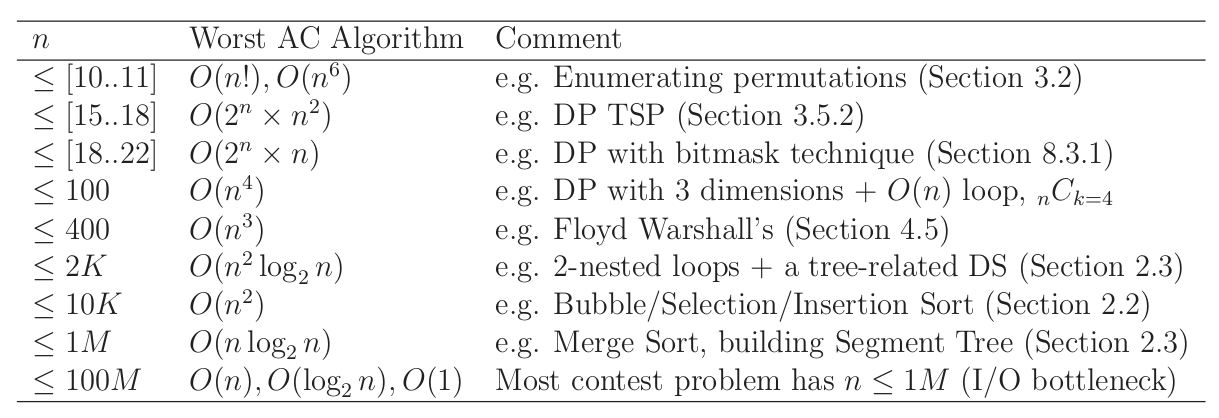
\includegraphics[scale=0.25]{imgs/1-CompetitiveProgramming/rule_of_thumb_complexities.png}
        \caption{Time complexities for a given $n$}
        \label{fig:my_label_20}
    \end{figure}
\end{frame}

%----------------------------------------------------------------------
%----------------------------------------------------------------------
%----------------------------------------------------------------------
\section{2. RAM Model and Big $O$ Notation}
\begin{frame}{Algorithm Analysis}
    \begin{itemize}
        \item Algorithms can be analyzed in a machine independent way
        \item We need techniques to compare the efficiency of algorithms before implementing them
            \begin{itemize}
                \item RAM Model
                \item Asymptotic Analysis - Big $O$ notation
            \end{itemize}
        \item Algorithms can be analyzed from two perspectives:
            \begin{itemize}
                \item \textbf{Time}: measured in units of time and represents the amount of time needed for an algorithm to complete
                \item \textbf{Memory}: measured in units of memory and represents the amount of memory used by the algorithm 
            \end{itemize}
        \item \textbf{Time} and \textbf{Memory} have an indirect relationship. Usually if we want less time we need more memory and viceversa
    \end{itemize}
\end{frame}

\begin{frame}{AA - The RAM Model}
    \begin{quote}
        In the RAM model we measure run time by counting the number of steps an algorithm takes on a given problem instance \\
            - Skiena \cite{skiena}
    \end{quote}
\end{frame}

\begin{frame}{AA - The RAM Model}
    \begin{itemize}
        \item Machine independent algorithms depend on a hypothetical computer called \textit{Random Access Machine}
        \item Each single operation ($+, -, *, \/, =, \text{if}$) takes one time step
        \item Loops and subroutines are a composition of multiple single operations. The time step of a loop depends on the number of iterations the loop makes
        \item Each memory access takes exactly one time step
    \end{itemize}
\end{frame}

\begin{frame}{AA - The RAM Model}
    \begin{figure}
        \centering
        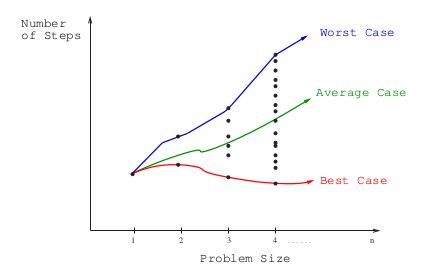
\includegraphics[scale=0.5]{imgs/1-CompetitiveProgramming/best-worst-avg-case.png}
        \caption{Best, Worst and Avergae case - See: \cite{skiena}}
        \label{fig:my_label}
    \end{figure}
\end{frame}

\begin{frame}{AA - Big $O$ notation}
    \begin{itemize}
        \item Provides a better intuition than the RAM Model since it:
            \begin{itemize}
                \item Require too much detail to specify precisely its behavior
                \item Many times the steps count depends on the programmer
            \end{itemize}
        \item Big $O$ notation solves this issues by providing upper and lower bounds of time-complexity functions
        \item Big $O$ notation ignores multiplicative constants
            \begin{itemize}
                \item $f(n) = 2n$ is considered the same as $g(n) = n$
            \end{itemize}
    \end{itemize}
\end{frame}

\begin{frame}{AA - Big $O$ notation}
    \begin{figure}
        \centering
        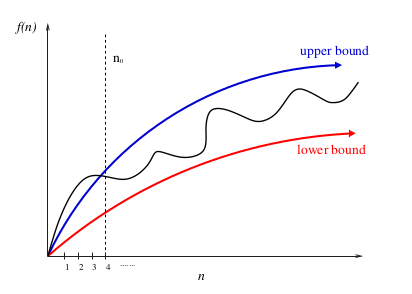
\includegraphics[scale=0.5]{imgs/1-CompetitiveProgramming/big-O-notation.png}
        \caption{Upper and lower bounds valid for $n>n_0$}
        \label{fig:my_label}
    \end{figure}
\end{frame}

\begin{frame}{AA - Big $O$ notation}
    \begin{figure}
        \centering
        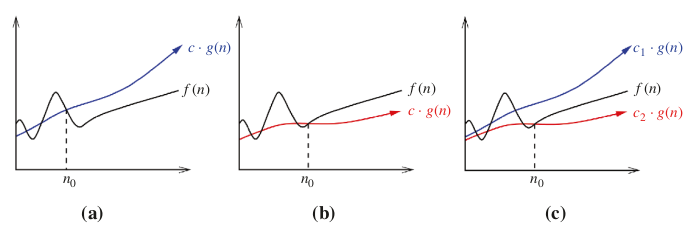
\includegraphics[scale=0.4]{imgs/1-CompetitiveProgramming/big-O-comparison.png}
        \label{fig:my_label}
    \end{figure}
    \begin{itemize}
        \item \textbf{a)}: $f(n) = O(g(n))$ $$f(n) \leq c\cdot g(n)$$
        \item \textbf{b)}: $f(n) = \Omega(g(n))$  $$f(n) \geq c\cdot g(n)$$
        \item \textbf{c)}: $f(n) = \Theta(g(n))$  $$c_2\cdot g(n) \leq f(n) \leq c_1\cdot g(n)$$
    \end{itemize}
\end{frame}

\begin{frame}{AA - Big $O$ notation: Examples}
    We want to identify $g(n)$ from $f(n)$:
    \begin{table}[H]
        \centering
        \begin{tabular}{|c|c|c|c|}
            \hline
            $f(n)$ & Possible $g(n)$ & Test with $c$ & Result \\ \hline
            $3n^2-100n+6$ & $n^2$ & $f(n) < 3n^2$ & $f(n) = O(n^2)$ \\ \hline
        \end{tabular}
    \end{table}
\end{frame}

\begin{frame}{AA - Big $O$ notation: Examples}
    We want to identify $g(n)$ from $f(n)$:
    \begin{table}[H]
        \centering
        \begin{tabular}{|c|c|c|c|}
            \hline
            $f(n)$ & Possible $g(n)$ & Test with $c$ & Result \\ \hline
            $3n^2-100n+6$ & $n^2$ & $f(n) < 3g(n)$ & $f(n) = O(n^2)$ \\ \hline
            $3n^2-100n+6$ & $n^3$ & $f(n) < 1g(n)$ & $f(n) = O(n^3)$ \\ \hline
            $3n^2-100n+6$ & $n$ & $f(n) > g(n)$ & $f(n) \neq O(n)$ \\ \hline
        \end{tabular}
        \caption{Tests for $O$}
    \end{table}
\end{frame}

\begin{frame}{AA - Big $O$ notation: Examples}
    We want to identify $g(n)$ from $f(n)$:
    \begin{table}[H]
        \centering
        \begin{tabular}{|c|c|c|c|}
            \hline
            $f(n)$ & Possible $g(n)$ & Test with $c$ & Result \\ \hline
            $3n^2-100n+6$ & $n^2$ & $f(n) > 2g(n)$ & $f(n) = \Omega(n^2)$ \\ \hline
        \end{tabular}
    \end{table}
\end{frame}

\begin{frame}{AA - Big $O$ notation: Examples}
    We want to identify $g(n)$ from $f(n)$:
    \begin{table}[H]
        \centering
        \begin{tabular}{|c|c|c|c|}
            \hline
            $f(n)$ & Possible $g(n)$ & Test with $c$ & Result \\ \hline
            $3n^2-100n+6$ & $n^2$ & $f(n) > 2g(n)$ & $f(n) = \Omega(n^2)$ \\ \hline
            $3n^2-100n+6$ & $n^3$ & $f(n) < g(n)$ & $f(n) \neq \Omega(n^3)$ \\ \hline
            $3n^2-100n+6$ & $n$ & $f(n) > g(n)$ & $f(n) = \Omega(n)$ \\ \hline
        \end{tabular}
        \caption{Tests for $\Omega$}
    \end{table}
\end{frame}

\begin{frame}{AA - Big $O$ notation: Examples}
    We want to identify $g(n)$ from $f(n)$:
    \begin{table}[H]
        \centering
        \begin{tabular}{|c|c|c|c|c|}
            \hline
            $f(n)$ & Possible $g(n)$ & Test with $c$ & Result \\ \hline
            $3n^2-100n+6$ & $n^2$ & Both $O$ and $\Omega$ apply & $f(n) = \Theta(n^2)$ \\ \hline
            $3n^2-100n+6$ & $n^3$ & $\Theta$ does not apply & $f(n) \neq \Theta(n^3)$ \\ \hline
            $3n^2-100n+6$ & $n$ & $O$ does not apply & $f(n) \neq \Omega(n)$ \\ \hline
        \end{tabular}
        \caption{Tests for $\Theta$}
    \end{table}
\end{frame}

\begin{frame}{AA - Big $O$ notation: Dominance Relations}
    \begin{itemize}
        \item Big $O$ notations groups functions into a set of classes such that all functions within a particular class are essentially equivalent
            \begin{itemize}
                \item $f(n) = 230n$ is equivalent to $g(n) = 1.5n$
                \item Both $f(n)$ and $g(n)$ belong to $\Theta(n)$
            \end{itemize}
        \item A faster growing function dominates a slower growing one
            \begin{itemize}
                \item We say that $g(n)$ dominates $f(n)$ when $f(n) = O(g(n))$
                \item $g \gg f$
            \end{itemize}
    \end{itemize}
\end{frame}

\begin{frame}{AA - Big $O$ notation: Function Classes I}
    Remember that we always need to measure the performance of our function when $n \to \infty$
    \begin{itemize}
        \item \textit{Constant functions}, $f(n) = 1$: no dependence between $f$ and $n$. Might measure the cost of adding two numbers, obtaining $\min$, $\max$, $\dots$
        \item \textit{Logarithmic functions}, $f(n) = \log n$: $f$ grows slowly as $n$ gets big but grows faster than the constant function. 
        \item \textit{Linear functions}, $f(n) = n$: might measure the cost of looking at each item in an $n$-element array.
        \item \textit{Superlinear functions}, $f(n) = n\log n$: grow a little faster than linear and might measure the cost of sorting an $n$-element array
    \end{itemize}
\end{frame}

\begin{frame}{AA - Big $O$ notation: Function Classes II}
    \begin{itemize}
        \item \textit{Quadratic functions}, $f(n) = n^2$: measure the cost of looking at most or all pairs of items in an $n$-element universe (array, sets, lists, $\dots$)
        \item \textit{Cubic functions}, $f(n) = n^3$
        \item \textit{Exponential functions}, $f(n) = c^n$: for a given constant $c>1$. Might measure the cost when enumerating all subsets of $n$ items
        \item \textit{Factorial functions}, $f(n) = n!$: measure the cost of generating all permutations or orderings of $n$ items
    \end{itemize}
\end{frame}

\begin{frame}{AA - Big $O$ notation: Dominance relations}
    $$n! \gg 2^n \gg n^3 \gg n^2 \gg n\log n \gg n \gg \log n \gg 1$$
\end{frame}

\begin{frame}{AA - Running time of common function classes}
    \begin{figure}
        \centering
        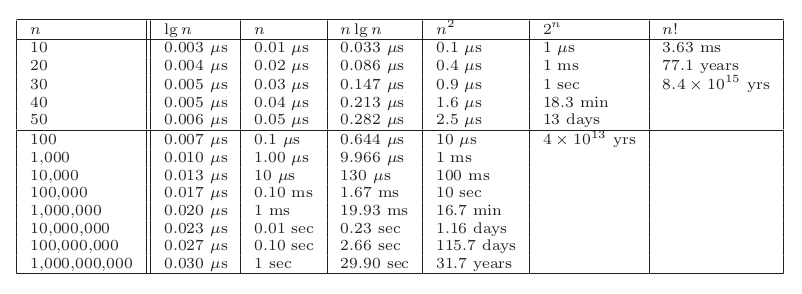
\includegraphics[scale=0.4]{imgs/1-CompetitiveProgramming/running-time-ns.png}
        \caption{Running time of function classes in nano seconds}
        \label{fig:my_label}
    \end{figure}
\end{frame}

%----------------------------------------------------------------------
%----------------------------------------------------------------------
%----------------------------------------------------------------------
\section*{References}
\begin{frame}{References}
    \begin{thebibliography}{}
        \bibitem[Halim]{Halim} Halim S., Halim F., \textit{Competitive Programming 3}, Handbook for ACM ICPC and IOI Contestants. 2013
        \bibitem[Stroustrup]{Stroustrup} Stroustrup B. \textit{The C++ Programming Language}. Fourth ed. 
        \bibitem{skiena} Skiena S. \textit{The Algorithm Design Manual}. Springer. 2020
    \end{thebibliography}
\end{frame}

\end{document}













